\documentclass[border=4mm]{minimal}
\usepackage{tikz}
\usetikzlibrary{positioning,shadows,shapes,arrows,calc}

\tikzset{abstract/.style={rectangle, draw=black,
    rounded corners, fill=blue, drop shadow,
    text centered, text=white, anchor = north, text width=3cm,
    text justified,rectangle split, rectangle split parts=2},
  myarrow/.style={->, >=open triangle 90, thick},
  line/.style={-, thick}
}

\begin{document}

Use \textbf{anchor} to make sure that the nodes is align on the top

\hfill

\begin{center}
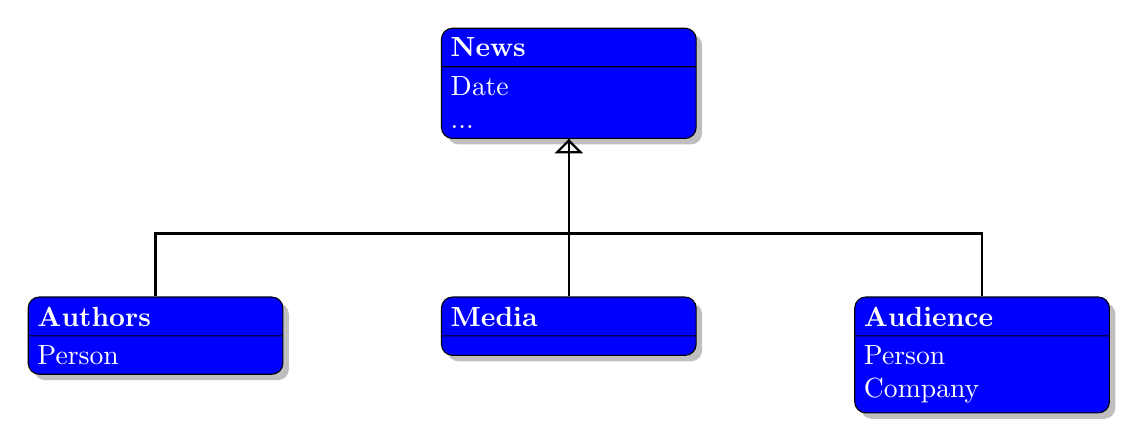
\begin{tikzpicture}[node distance=2cm]

   %Person node
   \node (Node-A) [abstract, rectangle split, rectangle split parts=2]
   {
      \textbf{News}
      \nodepart{second}Date\newline ...
   };

   %Media node
   \node (Node-B) [abstract, rectangle split, rectangle split parts=2, below=of Node-A]
   {
      \textbf{Media}
      \nodepart{second}
   };

   %Authors node and use anchor
   \node (Node-B-1) [abstract, rectangle split,
   rectangle split parts=2, left=of Node-B.north west,anchor=north east]
   % place node to north west of Node-B and using anchor is Node-B at north east
   {
      \textbf{Authors}
      \nodepart{second} Person
   };

   %Audience node and use anchor
   \node (Node-B+1) [abstract, rectangle split,
   rectangle split parts=2, right=of Node-B.north east,anchor=north west]
   {
      \textbf{Audience}
      \nodepart{second}Person\newline Company
   };

   \draw[line] (Node-B-1.north) -- ++(0,0.8) -| (Node-A.south);
   \draw[myarrow] (Node-B.north) -- (Node-A.south);
   \draw[line] (Node-B+1.north) -- ++(0,0.8) -| (Node-A.south);

\end{tikzpicture}
\end{center}

\hfill

Use \textbf{tree style} for the same type of diagram

\hfill

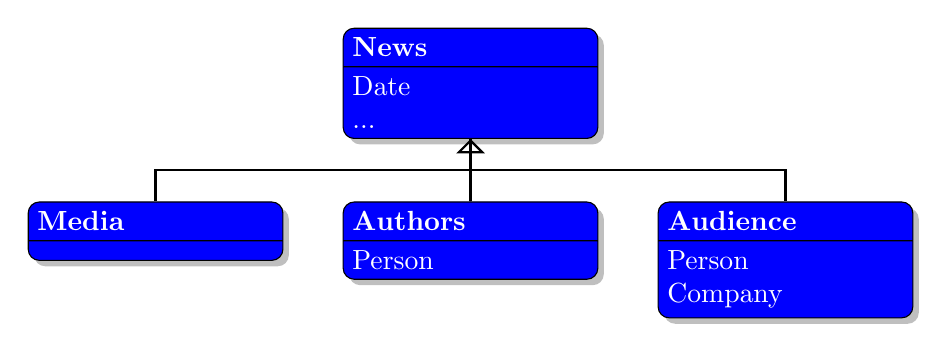
\begin{tikzpicture}[
  sibling distance=4cm,
  edge from parent path={
     (\tikzparentnode.south) --
     ($(\tikzparentnode.south)!0.5!(\tikzparentnode.south |- \tikzchildnode.north) $) -|
     (\tikzchildnode.north)},
  edge from parent/.append style={line}]

   %Person node
   \node (toplevel) [abstract]
   {
      \textbf{News}
      \nodepart{second}Date\newline ...
   }
   %Media node
  child {  node [abstract]
   {
      \textbf{Media}
      \nodepart{second}
   }
   }
   %Authors node
   child {node [abstract]
   {
      \textbf{Authors}
      \nodepart{second} Person
   }
   }
   %Audience node
   child { node (Node-B+1) [abstract]
   {
      \textbf{Audience}
      \nodepart{second}Person\newline Company
   }};

\draw [myarrow] (toplevel-2) -- (toplevel);

\end{tikzpicture}

\end{document}